\chapter{Програмна реализация}
\section{Избор и изграждане на базата данни}

Една система за езиково обучение очевидно се нуждае, най-малко, от
някакви речникови данни, на които тя да базира своите модули. Тези
данни трябва да бъдат съхраняване някъде. Много подобни системи
съхраняват данните си директно в текствови или двоични файлове. Това,
обаче, не е особено ефективно когато искате да правите произволен
достъп до данните или да манипулирате много от тях едновременно. 

Едно много по-ефективно решение е да се използва вградена релационна
база данни - подход използвам в много популярни приложение, като
Mozilla Firefox(SQLite), OpenOffice.org(HSQLDB) и т.н. В света на Java
приложенията най-популярните вградени бази данни са HSQLDB, H2 и Apache
Derby(изестна още като Java DB). И трите са реализирани изцяло на Java
и се интегрират отлично с Java приложения. В настоящата дипломна работа H2
Database беше предпочетена поради изключително високото си
бързодействие, малкият размер оперативна памет, която тя използва,
отличната си документация, чести обновления и леснота на употреба.

За да бъде тя достъпна в приложението трябва да се изпълнят следните
стъпки: 
\begin{itemize}
  \item h2.jar трябва да бъде добавен в клас пътя на приложението 
  \item за достъп се използва JDBC драйвера org.h2.Driver
  \item използва се URL за достъп до базата от вида
    jdbc:h2:/path/to/file
  \item ако базата не съществува тя ще бъде създадена първия път,
    когато се свържете към нея
\end{itemize} 
\section{Моделиране на базата данни}

Дизайнът на базата данни на приложението е изчистен, интуитивен и
минималистичен. Основните таблици, в които се съхраняват данните му са
само 5 - DICTIONARIES, DICTIONARY\_ENTRIES, STUDY\_SETS,
STUDY\_SET\_ENTRIES, RANK\_ENTRIES и EXAM\_SCORE\_ENTRIES. Всичките
съдържат няколко общи полета - уникален идентификатор(id), дата на
създаване(created), дата на промяна(modified). Общите полета в
таблиците са изразени в Java кода под формата на абстрактен базов
клас, който всичко други класове от бизнес модела разширяват. 

Таблицата DICTIONARIES съдържа следната информация - име на речник,
име на иконката на речника, двата езика, които го
описват(from\_language, to\_language). Добавянето на нов речник в
системата неминуемо минава през добавянето на нов ред в тази таблица. 

Таблицата DICTIONARY\_ENTRIES съдържа в себе си думите на
речниците. Нейните полета включват дума, превод и референция към
речника, който притежава думата. Следва се ествествената логика, че
един речник притежава много думи.

Таблицата STUDY\_SETS съдържа информация за същестуващите набори от
думи за изучаване. Думите от в един набор трябва да бъдат от
единствен речник, затова таблицата притежава референция към речник.

Таблицата STUDY\_SET\_ENTRIES съдържа думи на един набор, които по
същество са просто препратки към DICTIONARY\_ENTRIES. Освен това имаме
и референция към STUDY\_SET таблицата.

В таблицата RANK\_ENTRIES се съдържа рейтинга на думите в даден
език. Думите с висок рейтинг са често срещани, а тези с малък -
рядко. Както бе упомената и в предната глава, таблицата се използва от
изпитния модул за разделяне на думите по трудности, а данните в нея са
базирани на статистически анализ проведен върху различни литературни
творби.

Таблицата EXAM\_SCORE\_ENTRIES служи за съхранение на резултатите от
положените изпити. В нея се съхранява следната информация - използван
речник, име, брой верни отговори, брой грешни отговори и трудност на
изпита. 
\section{Изграждане на потребителският интерфейс}

Приложението има графичен потребителски интерфейс, реализиран
посредством библиотеката Swing на Java. Присъстват типичните за
повечето приложения елементи като лента с менюта (menubar) и лента с
бутони за бърз достъп до фунции(toolbar). Освен това приложението се
интегрира със областта за нотификации на операционната система.

Особено голяма внимание беше отделено на създаването на аткрактивен и
интуитивен дизайн на потребителският интерфейс. Той бе преработвам
изцяло няколко пъти преди да достигне до текущия си вид. За
допълнително удобство на потребителите интерфейсът е достъпен на
български и на английски език(посредством Translator инфраструктурата
на проекта), като е много лесно добавянето на още езици. 

Swing поддържа концепцията на включваеми външни видове(pluggable look
\& feels) - те позволяват на едно Swing приложение да изглежда по
много различни начини - например като Windows приложение, GTK+
приложение и са начин да се стесни пропастта между Swing апликациите и
така наречените native апликации. Spellbook използва включваемите
външни видове и позволява на потребителя да избери този, който му
допада най-много.
\section{Обобщена архитектура на приложението}
\section{Модули на приложението}
Реализацията на приложението е разделена в четири модула - ядро(core),
помощни пособия(utils), Swing компоненти(swing), потребителски
интерфейс(ui). Модулите на приложението са ясно обособени и са
всъщност и Maven модули - относително автономни единици изходен код.  
\subsection{Ядро}
В модула "`Ядро"' е събрана най-общатата и преизползваема логика на
приложението. Тук е реализирана комуникацията с базата данни, бизнес
модела на приложението и логиката, която задвижва инструментите
"`Изпит"', "`Учене на думи"', "`Проверка на правопис"' и т.н. Вътрешно
модула е разделен на Java пакети, в които е групирана свързаната
логика. Модулът "`Потребителски интерфейс"' се нуждае от възможностите
предоставени от модула "`Ядро"'. Следва описание на някои от ключовите
класове в модула "`Ядро"'.

\begin{itemize}
  \item \textbf{Translator}

    Класът Translator предлага възможност за превод на низове на
    различни езици посредством ResourceBundle. Класът се използва
    изключително от потребителският интерфейс, за да реализира
    възможността той да същестува преведен на различни
    езици. Класът транслатор има private конструктор и неговите
    инстанции се създават чрез метод-шабрика(един от шаблоните за
    дизайн). За всеки ResourceBundle съществува точно една инстанция
    от тип Translator. Инстанциите от класа вътрешно се кешират и се
    преизползват, когато са необходими.

    Всички елементи на графичния потребителски интерфейс притежават в
    себе си инстанция от класа, посредством, която те превеждат
    низовете в тях. За промяна на езиковите на стройките е необходимо
    Spellbook да бъде рестартиран - по време на този процес всички
    съществуващи инстанции на класа биват ре-инициализирани с новите
    езикови настройки.
   
  \item \textbf{AbstractEntity}

    Класът AbstractEntity е много важен, тъй като той е базовият клас,
    който разширяват всички класове част от модела на
    приложението. Самият той е доста прост - съдържа само три полета,
    които са общи за всеки бизнес тип, а именно дата на
    създаване(created), дата на промяна(modified), уникален
    идентификационнен номер(id).

\begin{figure}[htbp]
  \caption{Диаграма на класовете от модела на приложението}
  \centering
  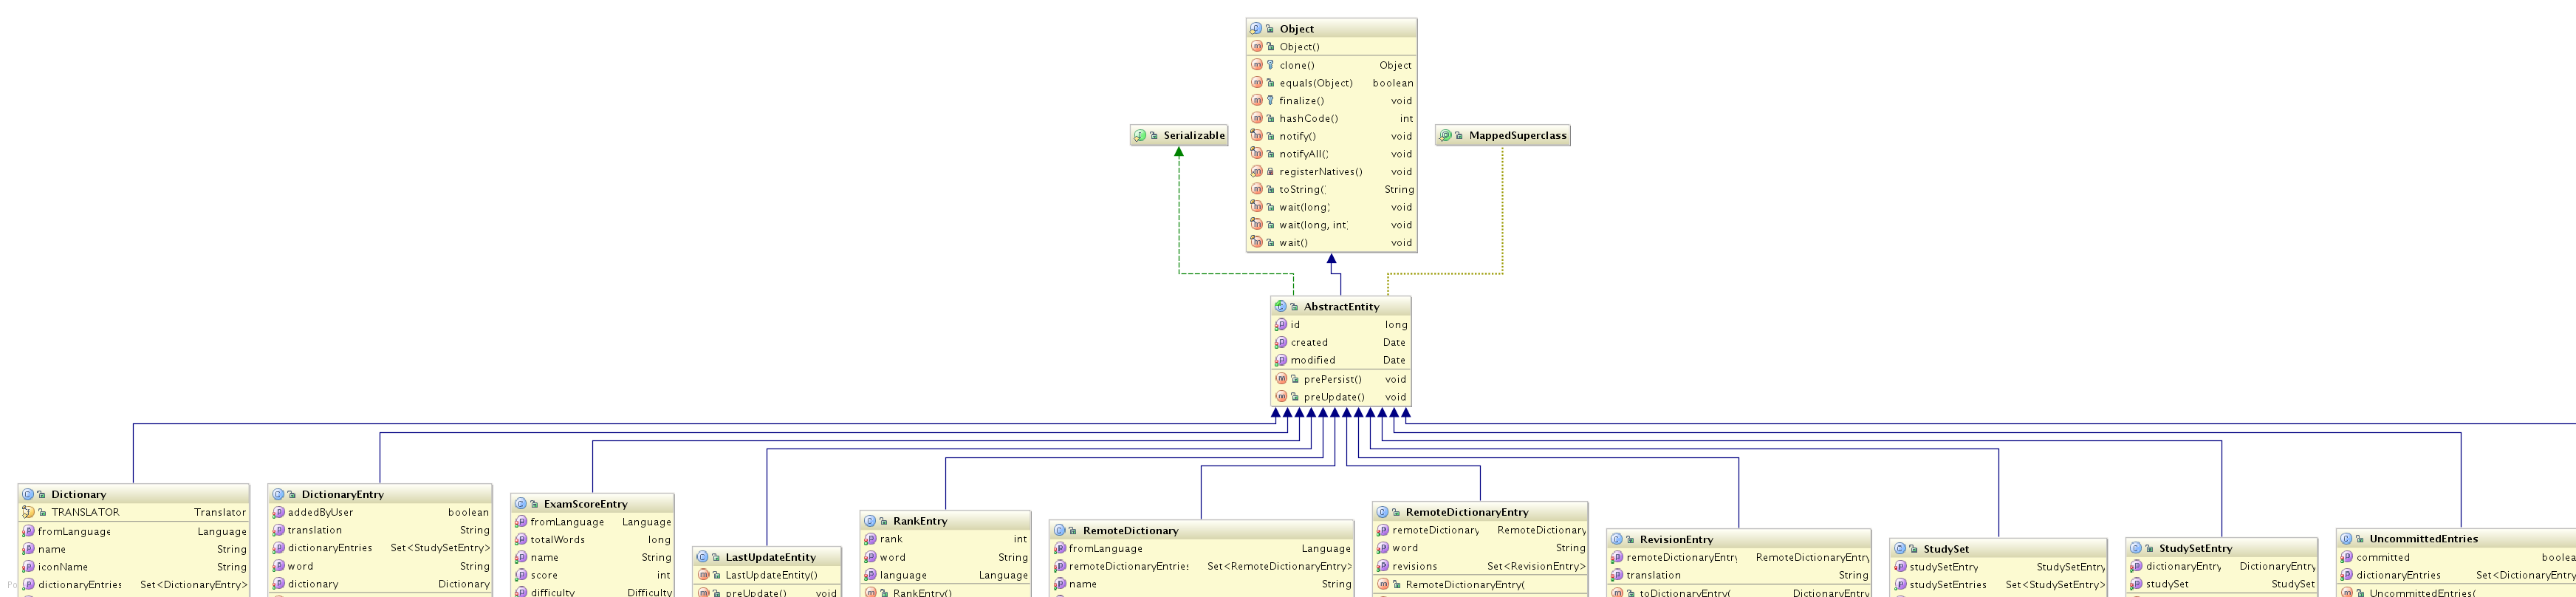
\includegraphics[width=110mm, height=40mm]{images/model-diagram.png}
\end{figure}

  \item \textbf{PreferencesManager}

    Приложението се нуждае от начин за съхранение на потребителските
    настойки между различните сесии и класът PreferencesManager го
    предоставя. Класък представявлява обвивка над стандартния Java
    клас Preferences - всички преференции се записват в единствен
    възел и броят им е ограничен от изброен тип(enum) Preference,
    което елиминира вероятността името на настройка да бъде сбъркана.

    Класът PreferencesManager имплементира шаблона на дизайн
    сек(singleton) - от него съществува единствена инстанция, която си
    споделят всички класове, които имат нужда от него. 

    Самото съхранение на преференциите зависи от операционната
    система, върху която използвате приложението - в Unix базирани
    операционни системи настойките се запазват в скрита папка в
    домашната директория на приложението, а под Windows - в Windows
    регистрите. 

  \item \textbf{AbstractPersistenceService}

    Класът предоставя базов достъп до базата данни на
    приложението. Достъпът се осъществевя посредством единствена
    инстанция от тим EntityManager, която се създава първият път,
    когато се използва класа. Тази инстанция е protected поне на класа
    и това позволява на класовете наследници лесен достъп до
    него. EntityMagager е клас от JPA и той дава възможно за
    извърване на операции създаване, обновяване, изтриване, прочитане
    на персистентни обекти(entities) и за изпълняване на JPQL и SQL
    заявки. Когато имплементацията на JPA, която се използва е
    Hibernate, както в настоящето приложение - класът вътрешно е
    реализиран, използвайки Hibernate Session класа.

    Всички класове, които имат нужда от достъп до базата данни трябва
    да разширяват AbstractPersistenceService. Примери за такива
    класове са DictionaryService, StudyService, ExamService.
  \item \textbf{DictionaryService}

    Класът предоставя достъп до речниците, налични в базата данни и е
    ключов, тъй като други класове, като StudyService и ExamService са
    изградени върху неговите възможните.

    Класът предоставя възможност за извършване на следните операции -
    извеждане на наличните речници, търсене на определен речник,
    изваждане на думите от определен речник, добавене на дума в
    речник, промяна на дума в речник, изтриване на дума от речник,
    проверка за комплементарност на речник, намиране на превод на дума
    от речник, намиране на приблизителен превод на дума от речник.

    Класът комуникира активно с базата данни и затова е естествено, че
    той наследява класът AbstractPersistenceService. Както и другите
    сервизни класове на приложение, DictionaryService е реализиран
    посредством шаблона сек. 

    Интересни подробности в реализацията на класа са воденето на
    подробен журнал(log) за случващите се събития и кеширането на
    речниците в паметта след първоначалото им зареждане. Подробният
    журнал прави лесно проследяването на работата на класа и опроставя
    много процесът на търсене на грешки, които неминуемо
    възникват. Кеширането на речниците пък подобрява многократно
    скороста на превключваме между речниците, които вече са били
    заредени. Първият път речниците трябва да бъдат прочетени от
    базата, която се намира на твърдият диск - това е бавен процес,
    затова копие на речника се казва в асоциативен масив(hash map) в
    оперативната памет. За цената на минимално количество повече памет
    скорост на зареждане на речниците при повторна нужда от тях се
    увеличава буквално в десетки пъти.
  \item \textbf{StudyService}

    Класът предоставя достъп до наборите от думи за учене. Той
    предлага възможност за създаване на набор, добавяне и изтриване на
    думи в него, както и изтриване на набор. Всичките тези операции са
    свързани с базата данни и затова класът разширавя базовия клас
    AbstractPersistenceService. Тъй като думите в наборите са думи от
    речници, класът се нуждае и от DictionaryService, който използва
    вътрешно.

    Както всички сервизни класове на приложението, StudyService е
    реализиран посредством шаблона за дизайн сек и притежава богат
    журнал на изпълнението си.
  \item \textbf{ExamService}

    Класът реализира функционалността необходима за провеждане на
    изпит, а именно разделяне на думите в един речник на нива на
    трудност, предоставяне на думи за изпит, проверка на верността на
    значенията им и записване на крайния резултат от проверждането на
    изпита. 

    Трудностите са дефинирани от изброимия тип Difficulty и имат имена
    и стойности, между които думите се считат за част от дадена
    стойност. Стойностите са определени статистически, чрез анализ на
    дълги художествени текстове на даден език. В процеса се създава
    асоциативна таблицата, ключовете на която са думите, а стойностите
    - броя пъти, в които дадена дума бива срещната. Асоциативния масив
    бива записам в базата данни като таблица(RankEntries). Всички
    получени стойности биват осреднени за да се определят подходящи
    нива за различните трудности. Рядко срещаните думи се маркират
    като трудни, а често срещаните като лесни.

    Преводът на всяка дума има обикновено повече от едно значение. При
    провеждането на изпита потребителя въвежда само по едно значение,
    като отговор на даден въпрос, затова преводите трябва да бъдат
    разделени интелигентно на всички потенциални значения, които могат
    да бъдат приети като отговор. Класът постига това чрез употребата
    на регулярни изрази.

    Тъй като класът достъпва активно базата данни, той също е
    наследник на базовия клас AbstractPersistenceService. Думите,
    използвани в изпитите, са част от речници и затова класът вътрешно
    използва активно инстанцията от класа DictionaryService.

    Както всички сервизни класове на приложението, ExamService е
    реализиран посредством шаблона за дизайн сек и притежава подробен
    журнал на изпълнението си.
  \item \textbf{Spellcheck}
    Функционалността за проверка на правописа е доста комплексна и
    понастоящем притежава две реализации в Spellbook. 

    Оригиналната имплементация е в класа MapSpellChecker и реализира
    прост алгоритъм за проверка на правописа, представен в една от
    статиите на популярният автор и разработчик Питър Норвиг(Peter
    Norvig). Тази имплементация се основа на статистически анализ на
    думите в голям текст на даден език за да се определят
    най-подходящите корекции и използва таблицата RankEntries, която
    се използва още и от ExamService. За съжаление алгоритъма се оказа
    много неефективен откъм употреба на системни ресурси - работи
    бавно и консумира много памет. Затова той бе заменен.

    Новата реализация на проверката на правописа се съдържа в класът
    HunSpellChecker. Той вътрешно използва популярната библиотека за
    проверка на правопис hunspell, използвана още в проекти като
    Google Chrome, OpenOffice.org и Mozilla Firefox. Тази реализация
    използва речниците на hunspell за проверката и работи много
    по-бързо и ефективно от оригиналната. Нейн минус е, обаче, че
    изисква употребата на JNI(Java Native Interface), тъй като
    hunspell е С библиотека и това донякъде нарушава портативността на
    приложението - налага се разпространението на различни негови
    версии, компилирани за различните процесорни микроархитектури.
    
    Както всички сервизни класове на приложението, MapSpellCheck и HunSpellCheck са
    реализирани посредством шаблона за дизайн сек и притежават подробен
    журнал на изпълнението си.
  \item \textbf{CodeHostingService}

    Класът предлага интеграция с услугите, предоставяни от Google Code
    и в частност възможност за създаване на доклад за грешка в
    системата за следене на грешки на проекта от потребителите
    директно от приложението. Вътрешно класът използва библиотеката на
    Google gdata за достът до Google Code.

    Както всички сервизни класове на приложението, CodeHostingService е
    реализиран посредством шаблона за дизайн сек и притежава подробен
    журнал на изпълнението си.

  \item \textbf{SyncService}

    Един от най-ключовите класове в Spellbook. Той осъществавя
    комуникацията между десктоп версията на приложението(настоящата
    дипломна работа) и уеб версията(разработена от колегата Иван
    Хантов). Комуникацията се осъществява посредством XML протокол,
    когато се изтегля списък думи от уеб приложението към десктоп
    приложението и посредством GET параметри добавени към заявката в
    обратната посока. 

    Spellbook изпраща на web приложението датата, на която е извършена
    последната синхронизация и получава като отговор XML документ
    съдържащ информация за промените думи от тогава до
    сега. Променените думи се записват в локалната база на
    приложението.

    Локално промените думи пък се изпращат една по една на уеб
    приложението по формата на заявки. Тези думи се трупат в опашката
    на уеб приложението, от където биват одобрявани/отхвърлени преди
    да станат глобално достъпни. 

    Библиотеката за обработване на XML, използвана от класа, е
    DOM(алтернативата и е SAX). Локалните речници биват обновени,
    посредством използването на инстанция от класа DictionaryService. 
\end{itemize}
 
\subsection{Помощни пособия}
В модула "`Помощни пособия"' имаме няколко класа, които са полезни
сами по себе си извън контекста на приложението, както и няколко малки
помощни приложения.
\begin{itemize}
  \item \textbf{Parser}

    Оригиналните речници за проекта бяха извлечени от свободната база
    данни от речници на проекта BgOffice. Неговите речници се
    разпространяват в двоичен формат и класът Parser реализира в себе
    си функционалността, необходима да се преобразува този двоичен
    формат доста текстов формат с кодировка UTF8, подходящ за
    импортиране в релационната база данни на проекта.
  \item \textbf{Importer}

    Класът Importer работи съвместно с класът Parser. Той импортира
    речниците от текстовия формат, създаден от Parser, в базата данни H2.
  \item \textbf{ArchiveUtils}

    Класът ArchiveUtils предоставя възможност за разархивиране на
    tar.bz2 архиви(в такъв формат се разпространява базата данни на
    Spellbook) посредством метода extractDbFromArchive. Подава му се
    път до архивен файл, който той първо декомпресира, а после
    разархивира. Вътррешно тези операции се реализират от библиотеката
    за работа с архиви на Apache Ant.
  \item \textbf{DateUtils}

    Класът DateUtil предоставя няколко метода за работа с дати, като
    например намирането на разликата между две дати или осредняване на
    група интервали от време. 
  \item \textbf{SearchUtils}

    Класът FindUtils по настоящем има само един метод -
    findInsertionIndex. Той посредством двоично търсене определя
    идекса, на който трябва да бъде добавена нова дума в даден
    речник.
  \item \textbf{CaseInsensitiveStringComparator}

    Класът имплементира интерфейсът Comparator за сравнява не низове,
    независи от големината на буквите в тях. Тази функционалност се
    използва при извеждане на думите от един речник, тъй като те не са
    сортиране вътрешно в базата данни.
\end{itemize}

\subsection{Swing компоненти}
В модула "`Swing компоненти"' е кода на някои Swing компоненти,
създане за нуждата на приложението, както и някои диалогови прозорци,
които не са част от основният потребителски интерфейс. Тук са също
така моделите и валидаторите за компонентите, използвани в
системата. Важно е да се отбележи, че всички диалогови прозорци в
Spellbook са наследници на класа StandardDialog от библиотеката
JideOSS, а не на стандарния JDialog компонент на Swing. StandardDialog
предлага по-прегледна структура на диалогов прозорец с три обособени
части - заглавна част, тяло и панел с бутони. Следва кратко изложение
на някои от ключовите класове в модула:


\begin{itemize}
  \item \textbf{DictionaryComboBox}

    Класът DictionaryComboBox реализира Swing компонент падащо меню за
    избор на речник. Той разширява стандартния JComboBox. Елементите в
    него са чувствителни към смяна на езика.
  \item \textbf{DifficultyComboBox}

    Класът DifficultyComboBox реализира Swing компонент падащо меню за
    избор на трудност. Той разширява стандартния JComboBox. Елементите в
    него са чувствителни към смяна на езика.
  \item \textbf{LanguageComboBox}

    Класът LanguageComboBox реализира Swing компонент падащо меню за
    избор на речник. Той разширява стандартния JComboBox. Елементите в
    него са чувствителни към смяна на езика.
  \item \textbf{ErrorDialog}

    Класът ErrorDialog реализира диалогов прозорец за грешка. Той се
    появява автоматично, когато възникне неочавана грешка в
    приложението и дава възможност на потребителя да разгледа
    събщението на грешката и нейния стек трейс(stack trace), както и
    да създаде автоматично доклад за грешка в системата за следене на
    грешки на проекта в Google Code.

    ErrorDialog се инстанцира автоматично от класът за обработка на
    грешки по подразбирене SpellbookDefaultExceptionHandler. 
  \item \textbf{IssueDialog}

    Класът IssueDialog реализира диалогов прозорец за създаване на
    доклад за грешка в системата за следене на грешки на проекта. Той
    е достъпен от диалога за уведомяване за грешки(ErrorDialog) и от
    менюто "`Помощ"' на програмата. 
  \item \textbf{SelectDbDialog}

    Класът SelectDbDialog реализира диалог, който дава на потребителя
    възможност да избере къде се намира базата при първото стартиране
    на приложението. Диалогът дава възможност базата да бъде изтеглене
    автоматично от интернет или да бъде избран пътя до нея в локалната
    файлова система.

    Диалоговият прозорец не позволява на потребителя да продължи преди
    да извърши едно от тези две действия. За услеснение на потребителя
    в полето на пътя до базата на локалната файлова система се
    използва overlay, който визуално указва дали е избрана валидна
    директория(такава, която съдържа архив на базата данни).
  \item \textbf{SpellbookDefaultExceptionHandler}

    Класът SpellbookDefaultExceptionHandler имплементира интерфейса
    UncaughtExceptionHandler и се грижи за обработката на непридвидени
    грешки по време на работата на приложението. Когато възникне
    такава грешка се извиква неговия метод uncaughtException, който
    показва диалога за грешка ErrorDialog.

    SpellbookDefaultExceptionHandler е инсталиран глобално за всички
    нишки на приложението в класът SpellbookApp.
  \item \textbf{WordOfTheDayDialog}

    Класът WordOfTheDayDialog реализира диалогов прозорец, който
    показва произволна дума от речника по подразбиране на
    приложението. Потребителя може да разглежда и повече думи, ако
    желае. Диалогът се отваря автоматично при стартиране на
    приложнието, ако е избрана настройката "`Показвай дума на деня при
    стартиране"'. Освен това е достъпен и от менюто "`Помощ"'.

  \item \textbf{ListBackedListModel}

    Класът ListBackedListModel реализира модел на JList компонент
    изграден върху Java List. Това е много по-гъвкав модел от
    стандартния, който използва масиви, тъй като списъците могат да
    бъдат разширавяни и свивани динамично. 
  \item \textbf{IconManager}

    Класът IconManager служи за работа с икони в приложението. Той
    представлява допълнително ниво на абстракция над стандартната
    работа с ресурси в Java приложенията. Използвайки подхода
    "`конвенция вместо конфигурация"' той открива файловете-икони само
    по тяхното име и размер. 

    Размерите за икони са предефинирани в класа в изброен тип IconSize
    и имат стойности 16х16, 24х24, 32х32 и 48х48 пиксела. 
  \item \textbf{SwingUtil}

    Класът SwingUtil съдържа няколко полезни статични метода, които
    реализират функционалност като показване на съобщения в балонче,
    форматиране на превод и изграждане на заглавен панел за диалогов
    прозорец. 
  \item \textbf{ButtonControllingDocumentListener}

    Класът ButtonControllingDocumentListener имплементира интерфейса
    DocumentListеner и асоциира състоянието на даден бутон с текущият
    документ. Когато в документът има текст бутонът е активен, а
    когато е празен - бутонът свързан с него е неактивен.
\end{itemize}
 
\subsection{Потребителски интерфейс}

Тъй като Spellbook е едно десктоп приложение с графичен потребителски
интерфейс е нормално да очакваме голяма част от кода му да бъде част
от модула "`Потребителски интерфейс"'. Това е факт - този модул е дом
на входната точка на приложението(класът SpellbookApp), основният
прозорец на приложението(класът SpellbookFrame) и всички диалогови
прозорци част от основният потребителски интерфейс. В следващите
редове ще направим им направим кратък преглед.


\begin{itemize}
  \item \textbf{SpellbookApp}

    Класът SpellbookApp е входната точка на приложението - в него се
    съдържа неговият main метод. При стартирането му се инициализират
    Translator и PreferencesManager инфраструктурите, контрола на
    екрана за зареждане не прехвърля от виртуалната машина към
    приложението, установавят се някои настройки, като например локала
    и външният вид, проверява се присъствието на базата данни и ако
    всичко е наред се показва главният прозорец на приложението(в
    случай, че не е избрана настройката "`Стартирай в трей"'.

    Показването на екрана за зареждане на приложението се извършва на
    два етапа. Първо, посредством специален запис в манифеста,
    генериран от Maven се извежда прост екран, който представлява само
    една картинка. Когато виртуалната машина бъде заредена, тази
    картинка бива прихваната и декорирана с лента показваща прогреса
    на зареждането. Принципно първата крачка може да бъде пропусната,
    но ако потребителя има по-бавна машина може да мине известно
    време, докато стартира неговата виртуална машина. В това време той
    би се чудил дали въобще се случва нещо. Използвайки специалната
    конфигурация за показване на екран за зареждане той се появява
    моментално при стартирането на приложението, преди още да е
    заредила виртуалната машина. 

    Ако проверката за наличието на базата данни пропадне потребителят
    бива подканен с диалоговия прозорец SelectDb да избере
    такава. Извършва се и проверка за версията на Java виртуалната
    машина - ако тя не е Sun Java на потребителя бива показано
    съобщение, което го предупреждава за потенциални проблеми с
    използваната от него виртуална машина. След като основната
    инициализация приключи SpellbookApp създава инстанция от класа
    SpellbookFrame и прехвърля контрола към нея(като първо показва
    думата на деня, ако съответната настройка е избрана).
  \item \textbf{SpellbookFrame}

    Класът SpellbookFrame е най-комплексният клас в цялото приложение
    и той реализира основният прозорец на приложението - той включва в
    себе си речниковата перспектива на Spellbook, лентата с менютата,
    лентата с бутоните за бърз достъп до функции и статус
    лентата. Лентата с бутоните и статус лентата не са задължителна
    част от интерфейса и потребителите могат да ги крият, ако желаят. 

    Самият речников изглед е изключително прост - изграден е само от
    един JSplitPane, два JPanel за двете му страни, едно текстово поле
    за търсене на дума, един списък за селектиране на дума и един от
    компонент от тип JTextArea за визуализиране на превода да
    намерената дума. За този прост интерфейс, обаче, се крие голямо
    количество код, който реализира много допълнителни възможности,
    които не са видими на пръв поглед. 

    Някои от по интересните възможности са накратко изложени тук:
    
    \begin{itemize}
      \item натискането на Enter в полето за търсене маркира текущата
        дума и позволява да я изтриете само с един клавиш - Delete
      \item думите въведине в полето за търсене се запазват при
        настискане на клавиша Enter. Потребителя може да прелиства
        историята с търсени думи и да се възползва от автоматично
        дописване, ако желае да търси думата, която вече е търсел
        отново.
     \item ако напишете дума, която не се съдържа в речника ще ви бъде
       показана, думата най-близка до нея
     \item ако запишете да пишете дума на езика на комплементарния
       речник на избрания, речните ще бъдат автоматично сменени
     \item ако кликнете два пъти върху дума в списъка с думи ще ви
       излезе диалог, в който може да я редактирате
     \item преводът е допълнително форматиран с html markup за да бъде
       по-прегледен и по-лесен за четене от потребителите
     \item размерът и позицията на главният прозорец се запомнят между
       стартирания на програмата
    \end{itemize}

    Трябва да се отбележи и интеграцията със системните трей и
    клипборд, която се предлага посредством класовете
    ClipboardIntegration и SpellbookTray. Те позволяват речника да се
    крие в трея и да се превеждат автоматично думи копирани в
    клипборда.

    SpellbookFrame е и входната точка към цялата останала
    функционалност на приложението - чрез лентата с менюта(JMenuBar) и лентата с
    бутони(JToolBar) може да бъде достъпен всеки негов компонент. 

    Класът вътрешно използва много от класовете на системата -
    Translator, PreferencesManager, IconManager, DictionaryService, 
    ClipboardIntegration, SpellbookTray и други. Както и в журналните
    класове и тук е наличен подробен журнал за работата на класа.

    \item \textbf{ClipboardIntegration}

      Класът ClipboardIntegration имплементира интерфейса
      ClipboardOwner и предлага интеграция със системния
      клипборд. За съжаления, поради ограничения в Java, тази
      интеграция далеч не е идеална. Например - нямаме механизъм за
      нотификация при промяна на съдържанието на клипборда,
      единствената налична нотификация, е за загуба на
      собственичеството му. Затова Spellbook прибягва до следния хак -
      той взема съдържанието на клипборда и го връща там непроменено
      като по този начин става негов собственик. Когато друго
      приложение промени нещо в него Spellbook реагира на съобщението
      "`загубена е собствеността над клипборда"' и повтаря процедурата
      изложена по-горе. Това има неприятния страничен ефект, че би
      повлияло на работата на приложения, които правят подобни
      неща. Като цяло такива приложения би трябвало да са много малко,
      затова в практиката реално това не представява проблем. 

      Когато низ пристигне в клипборда той се разделя на думи и
      първата от тях се превежда автоматично(като евентуално превода
      може да бъде показан и в системната област за нотификации в
      зависимост от настройките). Някои думи като URL адреси се
      игнорират автоматично.

      Класът е реализиран посредством шаблона за дизайн сек, притежава
      журнал и референция към главния прозорец на приложението за да
      може да извика негов метод, когато възникне събитие, изискващо това.
    \item \textbf{SpellbookTray}

      Класът SpellbookTray реализира интеграция на Spellbook със
      системната област за известия(известна още като system
      tray). Това включва иконка в областта за известия, както и
      възможността тя да бъде щракана с левия и десен бутон на
      мишката. Събитията генерирани от ляво щракане карат главния
      прозорец да се крие и появява, а събията генерирани с дясното
      предизвикват появата на контекстно меню.

      Реализацията на трей иконата в Java е платформено зависима и не
      е идеална на всички платформи. Например под Linux се използва
      Motiff библиотеката, вместо модерните GTK+ и QT и иконата и
      нотификациите свързани с нея изглеждат ужасно. Очаква се
      ситуацията да се подобри в Java 7.
    \item \textbf{PreferencesDialog}

      Класът PreferencesDialog реализира диалогов прозорец, в който
      могат да бъдат конфигурирани голяма част от настройките на
      приложението. Неговата структура представява JTabbedPane с 3
      секции - "`общи настройки"', "`шрифтове"' и "`изпит"'.

      При създаването си диалогът бива инициализиран с текущите
      стойности на настройките, посредством PreferencesManager. Някои
      от настройките достъпни в него, като промяната на езика на
      потребителския интерфейс, изискват рестарт за да влязат в сила.

      Когато потребителя потвърди промените си с натискане на бутона
      OK диалогът бива подаден на класа PreferencesExtractor, който го
      анализира. 
    \item \textbf{PreferencesExtractor}

      Класът PreferencesExtractor аналазира текущото състояние на
      диалог от тип PreferencesDialog и на базата на него установя
      стойностите на всички настойки посредством
      PreferencesManager. Това може да бъде направено и в самият
      PreferencesDialog, разбира се, но разделението на
      задачите(separation of concerns) прави кода на PreferencesDialog
      по-чист и ясен.

      PreferencesExtractor води много подробен журнал за състоянието
      на всички настройки.
    \item \textbf{ExamDialog}

      Класът ExamDialog реализира диалогов прозорец за провеждане на
      изпит. Той е изграден от елементи за конфигуриране на изпита -
      като езика от който да се превежда и езика на който да се
      превежда(езиците, които са позволени зависят от наличните
      речници в речниковата база данни). Езиците и трудността на
      изпита по подразбиране биват инициализирани от текущите
      настройки.

      Изпитът има два вариант с време и без време - в зависимост от
      избраните настойки. Когато е избран изпит без време лентата с
      прогреса на времето за отговор е скрита. Изпитите могат да бъдат
      временно спрени и продължени в последствие. Настройките на
      изпита са достъпни посредством бутон в неговия диалогов
      прозорец, но само при положение, че изпитът е спрян в
      момента. Дължината на всеки изпит се определя в брой думи, които
      се конфигурират в неговите настойки. Времето за отговор на
      въпрос при изпит с време е зададено в инстанциите от изброения
      тип Difficulty - 45 секунди за ниска трудност, 30 секунди за
      средна и 15 секунди за висока. Ако потребителят не отговори на
      въпрос в рамките на определеното време текущият въпрос се счита
      за сгрешен и се преминава към следващият.

      Двигателят на изпитния диалог, разбира се, е класът
      ExamService. Изпитния диалог го използва за да придобие списък с
      думи съответстващи заданените изпитни настойки и за проверка на
      потребителските отговори. Класът използва и други от основните
      класове на приложението, а именно DictionaryService, Translator,
      PreferencesManager. 

      При приключване на изпита се показва инстанция от класа
      ExamSummaryDialog, където потребителя има възможност да прегледа
      представянето си по време на изпита и да запише своя резултат в
      базата данни, ако желае.
    \item \textbf{StudyDialog}

      Класът StudyDialog реализира диалогов прозорец, предоставящ
      възможността за изучаване на думи. Потребителя има възможност да
      избере набор от думи, които да изуча и реда, в който те да му
      бъдат представени. Допълнително потребителя има възможност да
      промени съществуващ набор от думи или да създаде нов такъв,
      което се случва в инстанция от класа WordsDialog. 

      В диалоговият прозорец WordsDialog потребителят може да
      манипулира набор от думи според избран речник. За улеснение на
      потребителите е реализирано автоматично дописване на думите в
      речника, с който той работи в момента.

      Класът StudyDialog използва вътрешно класа StudyService, а
      класът WordsDialog използа DictionaryService.

      Понастоящем настойките на модула "`учене на думи"' са
      интегрирани директно в него, но в бъдеща версия вероятно ще
      бъдат изтеглени в общата конфигурация на приложението.

    \item \textbf{HangmanDialog}

      Класът HangmanDialog реализира диалогов прозорец, който по
      същество представлява популярната игра
      "`Бесеница"'. Потребителят избира речник и ниво на трудност,
      след което старира играта. Бива му показана картинка на бесило и
      маскирана дума, буквите на която са заменени с
      подчертавки. Потребителят има възможност да гадае букви в
      думата(или цялата дума наведнъж). Ако познае буква тя бива
      показана в маскираната дума, а в противен случай се рисува
      елемент от картинката изобразяваща човек на бесило. Потребителят
      има право на 7 грешни опита преди да загуби играта. Играта от
      своя страна приключва успешно, когато потребителя разгадае
      маскираната дума. За помощ, при разгадаването на дума, на
      потребителите бива предоставено първото значение на думата.

      Алгоритъмът за определяне на трудностите в играта бесеница е
      същият, какво и в изпитния модул. Всъщност HangmanDialog
      вътрешно използва класа ExamService. Това е поредният примерно,
      който показва предимствата от разработката на преизползваеми
      класове.

      Графиката, показвана в играта се чертае от класа HangmanDrawing,
      който по същество е контейнер компонент, в който имаме инстанция
      от класа Graphics2D, посредством, която се изчертава
      картинката. Полето stage на класа указва до къде да се рисува
      графиката и се задава от HangmanDialog. 

    \item \textbf{AboutDialog}

      Класът AboutDialog реализира диалогов прозорец, в който е видима
      обща информация за приложението - неговата текуща версия,
      лиценз, екип, домашна страница.

      Всичките са достъпни посредством бутони в долната част на
      диалога. Натискането на бутона за показване на лиценза го отваря
      в браузъра по подразбиране - лиценза е дълът html документ и бе
      счетено за непрактично да бъде показан в самото
      приложение. Секцията с екипа на проекта пък дава възможност за
      изпращане на писма до членовете му.

      Налична е и връзка към официалния сайт на проекта, натискането
      на която също предизвиква отварянето на браузъра по
      подразбиране. Освен от главното меню този диалогов прозорец е
      достъпен и от иконата на приложението в областта за известия.

   \item \textbf{SpellCheckFrame}

     Класът SpellCheckFrame реализира прозореца на проверката на
     правописа. Той е единственият компонент от приложението освен
     SpellbookFrame, който има отделен прозорец. Причината за това е
     проста - напълно е възможно потребителят да иска да ползва
     едновременно проверката на правописа и речника едновременно. 

     Прозорецът за проверка на правописа има изключително прост дизайн
     - меню, в което да бъде избран език и голям текстов компонент, в
     който да бъде въведен текста, който искаме на да проверим. Когато
     бъде въведен текст грешките в него веднага биват подчертани с
     червени линии, а ако потребителя кликне върху някоя от
     сгрешението думи ще му бъдат предложени думи, с които да я
     замени. При селектиране на някоя от тези думи - тя заменя
     сгрешената дума. 

     В сърцето на прозореца за проверка на думи е сервизният клас
     HunSpellChecker, който по настоящем предоставя необходимата
     инфраструктура за проверка на правопис.

     Подобно на речниковата перспектива проверката на правописа
     поддържа интеграция със системния клипборд - ако там бъде копиран
     текст докато проверката на правописа е включена този текст
     автоматично ще бъде поставен там.
   \item \textbf{ContextMenuMouseListener}

     Класът ContextMenuMouseListener предоставя контектно меню с
     действия "`Копирай"', "`Изрежи"' и "`Вмъкни"', което може да бъде
     добавено към всеки Swing компонент, който разширавя класа
     JTextComponent - такива са например JTextField, JTextArea,
     JTextPane. Менюто се появява при кликане в компонента с дясното
     копче на мишката. 

     Swing текстовите компоненти поддържат тези действия и по
     подразбиране, но само с клавишни комбинация, без менюта, с които
     повечето потребители са свикнали, което наложи добавянето на тази
     фунционалност. 
   \item \textbf{AddUpdateWordDialog}

     Класът AddUpdateWordDialog реализира диалогов прозорец за
     добавяне на нова дума в речник или редактирането на вече
     съществуваща такава. Диалога подканва потребителите да въведат
     думата, която желаят и всяко нейно ново значение по отделно. 

     Посредством употребата на DictionaryService диалогът предовратява
     добавянето на вече съществуващи думи и записва новите думи и
     корекциите на същестуващите думи в съответните речници.

     Този прост диалогов прозорец е ключов компонент от една от
     най-вълнуващите способности на системата, а именно
     синхронизацията с отдалечената база данни на уеб версията на
     системата, разработена от колегата Иван Хантов. Думите добавени и
     променени от потребителите се маркират специално в базата данни и
     при извършване на процеса синхронизация бивав изпратени на уеб
     приложението. 

     Диалогът е достъпен от менюто "`Редактирай"' и лентата с бутони,
     а фунционалността му за промяна на съществуваща дума е достъпна и
     посредством MouseListener в списъка с думи - кликването с мишката
     върху някоя дума там отваря диалога.
\end{itemize}


%%% Local Variables: 
%%% mode: latex
%%% TeX-master: "master"
%%% End: 
